\documentclass[12pt]{article}

\usepackage[spanish]{babel}
\usepackage[utf8]{inputenc}
\usepackage{graphicx}
\usepackage{geometry}
\usepackage{xcolor}
\usepackage{fancyhdr}
\usepackage{lastpage}
\usepackage{pdfpages}
\usepackage{listings}

\geometry{top=25mm,left=15mm,right=15mm,a4paper}

\pagestyle{fancy}
\fancyhf{}
\lhead{Seminario de Ciencias de la Computación A}
\cfoot{Página \thepage\ de \pageref{LastPage}}

\graphicspath{./}

\begin{document}
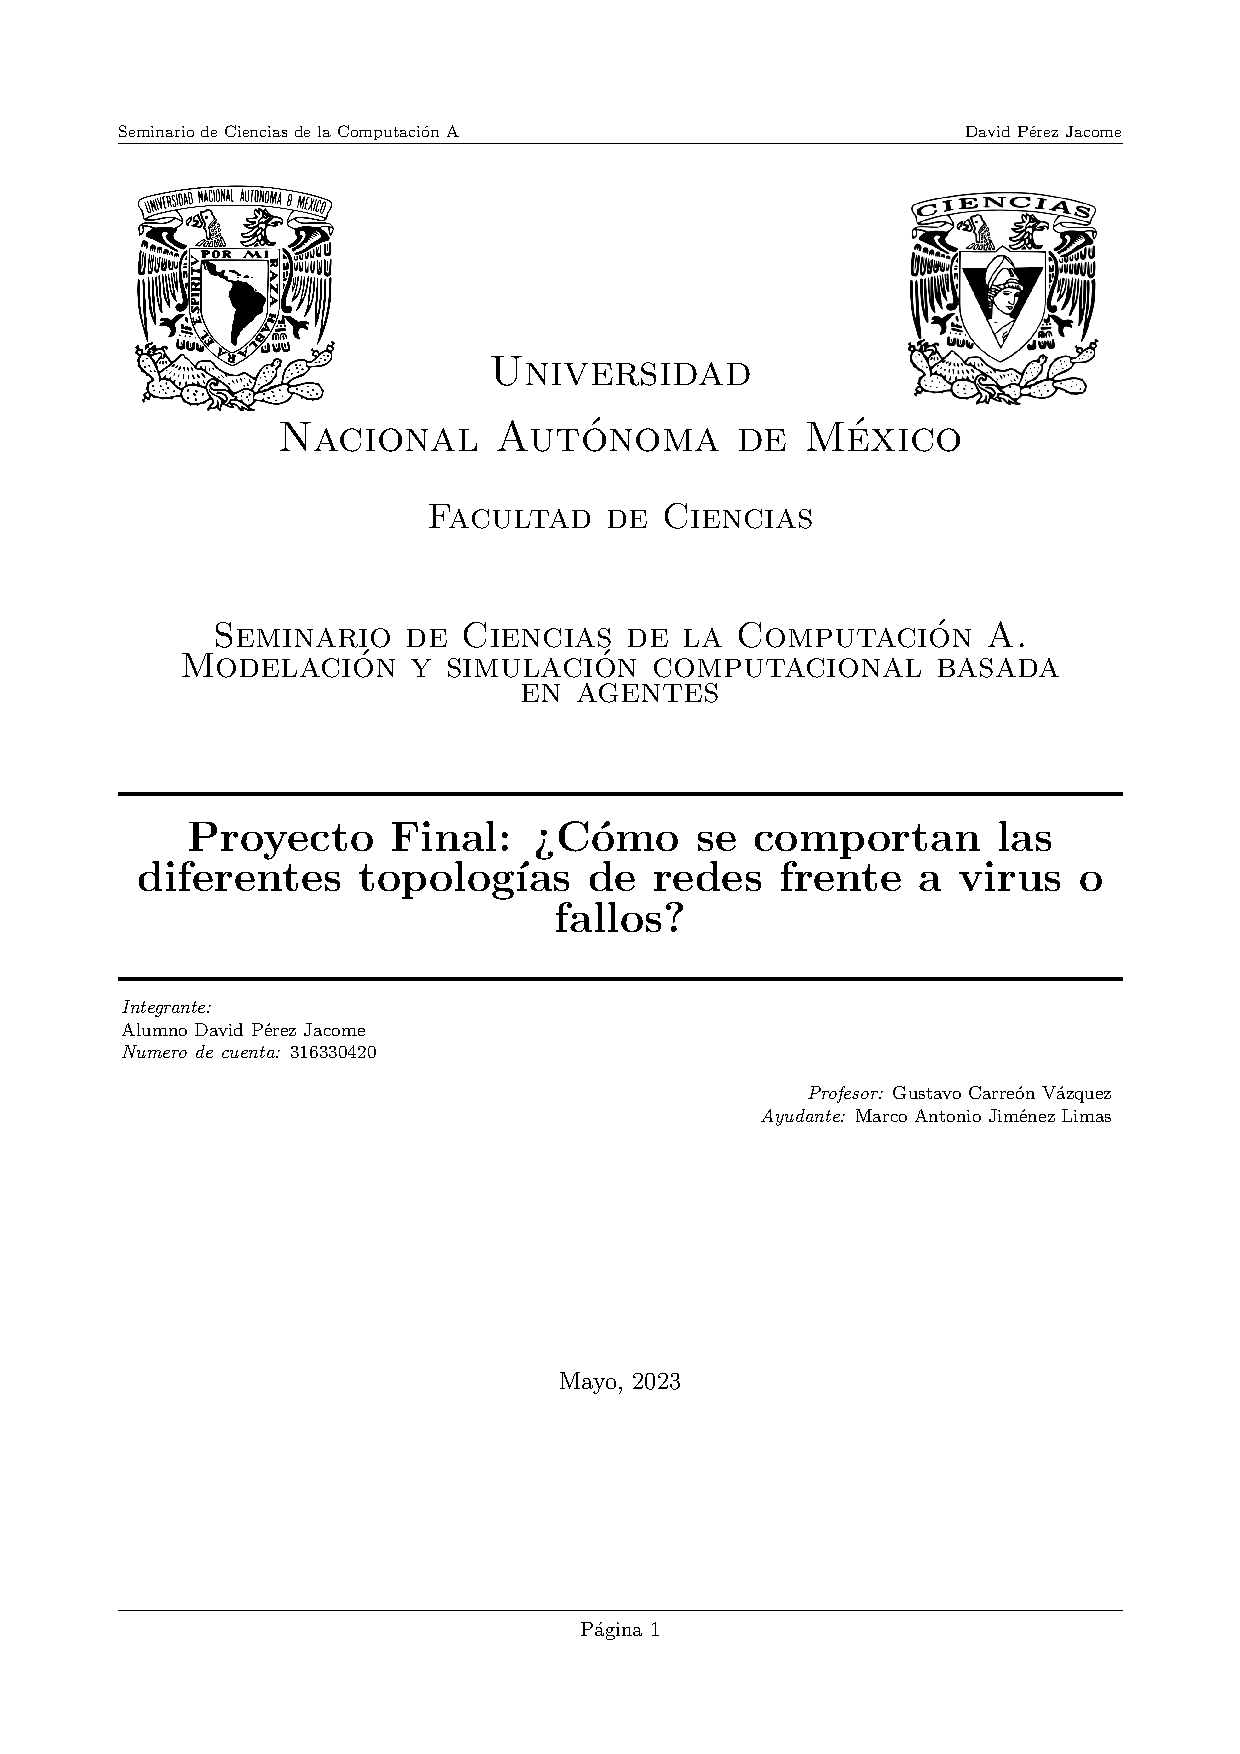
\includepdf{Portada.pdf}
{\color{red} \section*{Proyecto Final: ¿Cómo se comportan las diferentes topologías de redes frente a virus o fallos?.}}
\vspace{2em}

{\color{blue} \subsection*{1- INTRODUCCIÓN.}}
\vspace{1em}

¿Cómo se comportan las diferentes topologías de redes frente a virus o fallos?, esta es la pregunta a la que a lo largo de este trabajo nos vamos a dedicar a responder.
A lo largo del curso de Modelación Basada en Agentes hemos ido aprendiendo diversas aplicaciones y simulaciones del mundo real en las que podemos "modelar" y mostrar el como es el comportamiento de algún fenomeno
ya sea fisico o en este caso computacional, en este trabajo abordaremos principalmente la problematica de modelar una estructura de red, pero para ello debemos tener presente que es un sistema de redes, que en pocas palabras una red de ordenadores se refiere a dispositivos de computación 
interconectados que pueden intercambiar datos y compartir recursos entre sí. 
Los dispositivos de la red utilizan un sistema de reglas, llamados protocolos de comunicaciones, para transmitir información a través de tecnologías físicas o inalámbricas.\\

También veremos el comportamiento dado fallos en diferentes topologias de red, pero para esto debemos de tener presente que es la topología de redes, la topología de redes es la disposición de nodos y enlaces se denomina topología de red. Se pueden configurar de diferentes maneras para obtener diferentes resultados. Algunos tipos de topologías de red son:\\
\begin{enumerate}
    \item Bus: Cada nodo solo está vinculado a otro nodo. La transmisión de datos a través de las conexiones de red se produce en una dirección.
    \item Anillo: Cada nodo está vinculado a otros dos nodos, formando un anillo. Los datos pueden fluir de manera bidireccional. Sin embargo, el error de un solo nodo puede provocar la caída de toda la red.
    \item Estrella: Un nodo de servidor central está vinculado a múltiples dispositivos de red de clientes. Esta topología funciona mejor ya que los datos no tienen que pasar por cada nodo. También es más fiable.
    \item Malla: Cada nodo está conectado a muchos otros nodos. En una topología de malla completa, cada nodo está conectado a todos los demás nodos de la red.
\end{enumerate}

En las redes computacionales existen asi como diversos tipos de topologías, distintos tipos de fallos o infecciones via virus, para este proyecto nos enfocaremos principalmente en como se ve afectada la red dado un contagio que puede ser relacionado a un virus o a un fallo en el sistema, en general y para hacer un poco mas sencillo de entender y de implmenetar el sistema, vamos a utilizar un fallo similar a una infección via algún virus.
Pero es importante decir que no es lo mismo; Podemos definir los fallos o eventos de una red como aquellos sucesos que interfieren en el correcto funcionamiento de la red, y por consiguiente disminuyen significativamente su rendimiento. Los ejemplos de fallos más comunes incluyen fallos en el hardware, en el cableado, interferencia inalámbrica, así como un cambio en el estado del puerto, saturación de ancho de banda o, lo que es peor, la pérdida de conectividad.
Mientras que un virus informático es una aplicación o código malintencionado que se emplea para ejecutar actividades destructivas en un dispositivo o red local. La actividad malintencionada de este código puede dañar el sistema local de archivos, robar datos, interrumpir servicios, descargar más malware o cualquier otra acción que esté codificada en el programa. Muchos virus simulan ser programas legítimos para convencer a los usuarios de que los ejecuten en su dispositivo, insertando así la carga útil del virus.
En el que podemos de manera similiar utilizar el modelo SIR para su modelación.\\

Para este modelo nos apoyaremos de la biblioteca de modelos de NetLogo, el modelo \textbf{Virus on a Network} para no complicar tanto el modelo, de igualmanera por el tiempo y poder tener una base solida de la implementación.\\
Es importante modelar este tipo de comportamiento especifico en las redes ya que en ocaciones al tener una red de computadoras tan compleja como lo son la mayoria si no es que todas, y nos resulta que un componente de nuestro sistema tiene una falla, 
el como se debe de abordar tal problematica es de suma importancia para que el sistema siga con su proceso de comunicación apesar de la o las fallas que resulten, para que nuestro sistema no llegue a caer.\\

El modelar este tipo de comportamientos nos ayudan para saber el timpo de mantenimiento que le debemos de dar al sistema en si para que no ocacione fallas catastroficas que compromentan todo el sistema, asi mismo podemos ver en el modelo como es que se comunican los componentes del sistema a pesar de una falla o contagio.\\

En otros modelos que he visto este tipo de fallos los han abordado con distintos algoritmos distribuidos, estos algoritmos son también "Detectores de fallos", de igual manera es posible implmentar usando Modelación Basada en Agentes, este tipo de comportamiento de envio-recepción de mensajes. que trataremos de abordar de manera \textbf{implicita} en nuestro sistema.\\

En modelos basados en agentes este tipo de problemas de redes los han abordado de manera diferente, usando como lo mencione anteriomente diferentes tipos de algoritmos distribuidos, para esto explicaremos que es un algoritmo distribuido.
Un algoritmo distribuido es una colección de n autómatas, uno por proceso. Un autómata describe la secuencia de pasos ejecutados por el proceso correspondiente. Adicional al poder de una máquina de Turing, un autómata es enriquecido con dos operaciones de comunicación que permite enviar y recibir un mensaje en cualquier canal. Estas
operaciones son $send()$ y $receive()$.\\

Algunos de los algortimos que se utilizan son para detectar fallas en el sistema, algoritmos de detección de $k$ fallas, algoritmos que son tolerantes a fallas, algoritmos de conceso(los cuales se comunican los procesos entre si para llegar a una desición en común), estos mismos algoritmos de conceso pero con fallas en alguno de los componentes.
Como se puede leer, existen multiples aplicaciones y las mas practicas son los protocolos de red, en donde principalmente modelamos el sistema para ver como es que se comporta, también es importante para su estudio.\\

Existen muchas aplicaciones y muchos algoritmos de aplicación, sin embargo como lo mencionamos con anterioridad vamos a unir en la practica los conceptos de fallo con los de virus para una mejor y más facil implementación.\\

{\color{blue} \subsection*{2- PLANTEAMIENTO.}}
\vspace{1em}

{\color{red} \subsubsection*{2.1 Marco Teorico.}}
\vspace{1em}

En este proyecto vamos a analizar principalmente el comportamiento de los componentes computacionales, en este caso especificos supondremos que contamos con una serie computadoras interconectadas mediante la red, a este tipo de comunicaciones se les llama "Computación distribuida", el uso de estos componentes es de suma importancia en el aspecto de 
sincronización de estos componentes, suponiendo que tenemos un archivo en una base de datos lo debemos o lo podemos modificar de un componente y los demás deben de estar sincronizados entre si para que haya integridad en los datos e intercambio de ellos.
Para fines de la materia de Modelación Basada en Agentes vamos a usar la herramienta de \textbf{NetLogo} en la que vamos a tomar como punto de partida el modelo que pertenece a la biblioteca de modelos del programa, usaremos \textbf{"Virus on a
Network"}, no usaremos el modelo tal cual a como esta, lo modificaremos para que la topología del sistema se adapte a modelos mas realistas en donde los componentes están localizados de una manera aleatoria e incluso a distancias distintas.\\
En nuestea implementación usaremos tres estados base para nuestros componentes:\\
\begin{enumerate}
    \item Infectado: nuestro componente esta en estado infectado o en falla que por terminos del proyecto ambas las vamos a tomar como analogas aunque no lo son en realidad y cabe mencionarlo con determinación.
    \item Propenso a ser infectado: Es el estado inical de nuestro sistema y todos los componentes estan en riesgo de estar infectados o no.
    \item Recuperado o Salvado: En este estado, los componentes estan a salvo, puede que se hayan infectado pero despues de un determinado tiempo (ticks) el componente se recupera y ya no esta propenso a ser infectado o dañado. 
\end{enumerate}

En otros puntos más especificos en terminos del funcionamiento de nuestro modelo, tenemos varias particularidades, en primer aspecto tenemos sliders para poder determinar las distintas caracteristicas del modelo.\\
\begin{enumerate}
    \item \textbf{Probabilidad de infección:} probabilidad de infectar o que un nodo falle.
    \item \textbf{Tiempo de revisión de fallo:} tiempo (medido en ticks) que pase para checar si un nodo tiene algun fallo.
    \item \textbf{Probabilidad de recuperación:} la probabilidad de que un nodo se recupere del fallo o contagio.
    \item \textbf{Resistencis a fallos futuros:} despues de ser curado o reparado, el componente permanece inmune a fallos.
    \item \textbf{Grado minimo de un nodo:} número de aristas que salen de un nodo, el minimo es que es de este número en adelante.
    \item \textbf{Número de nodos:} número de componentes del sistema de redes.
    \item \textbf{Componentes fallidos:} número de componentes que inicializan el sistema con un fallo.
\end{enumerate} 

De igual manera es importante mencionar la topología de nuestro modelo, tomamos como topología inicialmete dos tipos, un tipo es topología de tipo \textbf{Distribución Circular}, en la que nos nodos estan esparcidos de manera de circulo al rededor de nuestro modelo.
También tenemos la topología \textbf{Topología Aleatoria} en esta topología nuestros nodos o componentes están repartidos sin restricciones en todo el mundo pueden formar distintas tipo de representaciones, esta representación es la más cercana a las del mundo real.\\

También es muy importante mencionar la comunicación de los componentes en el modelo, esta es otra de las variaciones respecto al modelo original, nuestro modelo tiene un tipo de comunicación de \textbf{Grafos Dirigidos}, esta su principal caracteristica es que son flechas dirigidas en las que los componentes solo se comunican en la dirección en la que se asocia su arista, no en otro sentido.

{\color{red} \subsubsection*{2.2 Objetivo General.}}
\vspace{1em}

El objetivo general de nuestro proyecto es:\\

\begin{enumerate}
    \item Ver y analizar el comportamiento de una red remota de distintos componentes que se localizan de manera aleatoria y el como dado un fallo en uno o más, como es que se comporta dicha red ante estos distintas
    problematicas y en que momento la red puede llegar a colapsar 
\end{enumerate}

{\color{red} \subsubsection*{2.3 Objetivos Especificos.}}
\vspace{1em}

Los objetivos especificos de nuestro proyecto parten del objetivo principal y son:\\
\begin{enumerate}
    \item Ver el comportamiento en distintas topologias lo mas cercanas a la realidad y su comunicación.
    \item Analizar el comportamiento de los componentes dados sus tres estados principales y el como se van modificando en respecto al tiempo.
    \item La distintas variaciones de los parametros y distintos ambientes en como se desenvuelve el sistema y en que momento puede llegar a un llamado "Fallo Total".
    \item La comunicación de los componentes y el analisis del como puede llegar a ser el sistema más eficiente sin importar el tipo de fallos o la cantidad.
\end{enumerate}


{\color{blue} \subsection*{3- DESARROLLO.}}
\vspace{1em}

En terminos generales las especificciones del programa las mencionamos en la sección anterior, pero ahora profundizaremos un poco más en los sliders, el mundo, y el funcionamiento de nuestro modelo.\\

\textbf{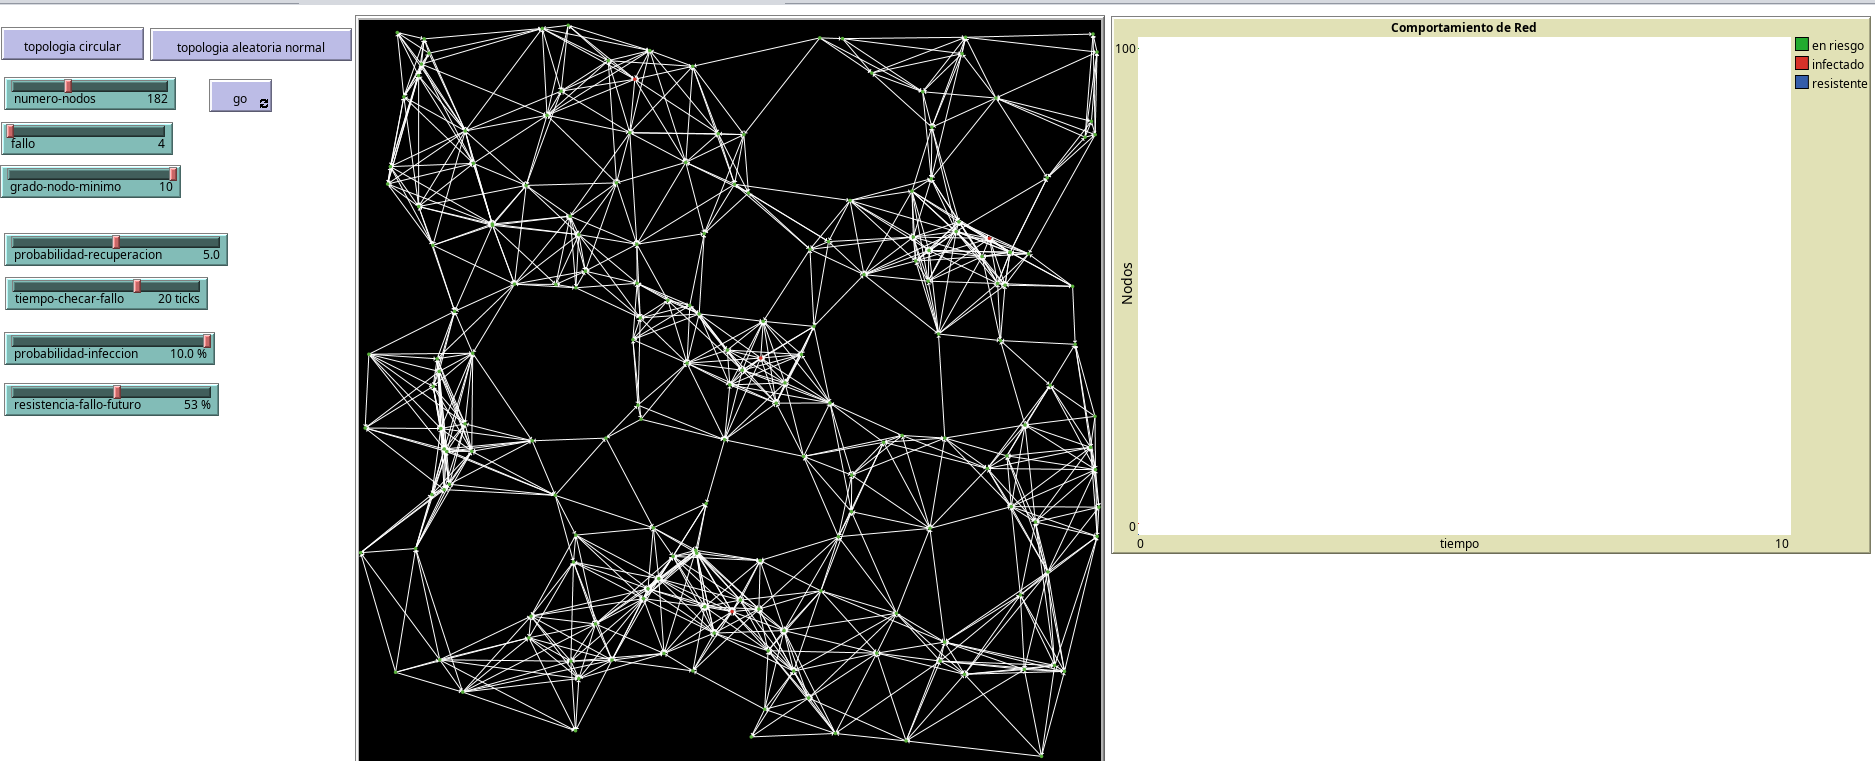
\includegraphics[scale = 0.30]{images/vista-general.png}}\\
Esta es la vista de nuestro modelo (tomando una topologia aleatoria).\\

Como podemos ver tenemos una serie de sliders:\\
\begin{enumerate}
    \item \textbf{Probabilidad de infección:} probabilidad de infectar o que un nodo falle. Va de $0$ a $10$
    \item \textbf{Tiempo de revisión de fallo:} tiempo (medido en ticks) que pase para checar si un nodo tiene algun fallo. de $0$ a $30$ ticks
    \item \textbf{Probabilidad de recuperación:} la probabilidad de que un nodo se recupere del fallo o contagio. de $0$ a $10$\%
    \item \textbf{Resistencis a fallos futuros:} despues de ser curado o reparado, el componente permanece inmune a fallos. de $0$ a $100$\%
    \item \textbf{Grado minimo de un nodo:} número de aristas que salen de un nodo, el minimo es que es de este número en adelante. número entero
    \item \textbf{Número de nodos:} número de componentes del sistema de redes. número entero
    \item \textbf{Componentes fallidos:} número de componentes que inicializan el sistema con un fallo. número entero
\end{enumerate}

También tenemos una grafica en la que mostramos con los colores asociados los 3 diferentes estados de los componentes o nodos:\\

\begin{enumerate}
    \item Infectado(\textbf{rojo}): nuestro componente esta en estado infectado o en falla que por terminos del proyecto ambas las vamos a tomar como analogas aunque no lo son en realidad y cabe mencionarlo con determinación.
    \item Propenso a ser infectado(\textbf{verde}): Es el estado inical de nuestro sistema y todos los componentes estan en riesgo de estar infectados o no.
    \item Recuperado o Salvado(\textbf{azul}): En este estado, los componentes estan a salvo, puede que se hayan infectado pero despues de un determinado tiempo (ticks) el componente se recupera y ya no esta propenso a ser infectado o dañado. 
\end{enumerate}

La grafica modela el comportamiento del sistema delante de diversas situaciones y es facil de ver si es que falla, en que casos es posible un colapso y en cuanto tiempo se puede llegar a recuperar el sistema.\\

Los algortimos vienen en la implementación del modelo pero para un facil comprendimiento los anexaremos acontinuación:\\

\begin{verbatim}
    ;; Funcion de inicialización setup, creamos los nodos y se conectan a topologia normal
to setup-b
  clear-all
  setup-grafo-aleatorio
  setup-red2
  ask n-of fallo turtles
    [ esta-infectado ]
  ask links [ set color white ]
  reset-ticks
end


;;setup crea los nodos del grafo de manera aleatoria (tomamos una topologia aleatoria)

to setup-grafo-aleatorio
  crt numero-nodos [
    setxy random-xcor random-ycor
    esta-en-riesgo
    set shape "circle"
    set color green
    set tiempo-fallo random tiempo-checar-fallo
  ]
end

;;setup para inicializar las conexiones de la red en topologia circular

to setup-red
 let numero-aristas (grado-nodo-minimo * numero-nodos) / 2
  while [count links < numero-aristas ]
 [
   ask one-of turtles
   [
      let eleccion (min-one-of (other turtles with [not link-neighbor? myself])
                     [distance myself])
      if eleccion != nobody [create-link-to eleccion ]
    ]
    repeat 10
    [
      layout-circle (sort turtles) max-pxcor - 1
    ]
  ]
end

;;setup para inicializar las conexiones de la red en topologia aleatoria

to setup-red2
  let numero-aristas (grado-nodo-minimo * numero-nodos) / 2
  while [count links < numero-aristas ]
 [
   ask one-of turtles
   [
      let eleccion (min-one-of (other turtles with [not link-neighbor? myself])
                     [distance myself])
      if eleccion != nobody [create-link-to eleccion ]
    ]
  ]
end



;;función que nos dice si esta infectado el nodo

to esta-infectado
  set dañado? true
  set resistente? false
  set color red
end

;;Funcion que nos dice si es posible dañar o contagiar el componente

to esta-en-riesgo
  set dañado? false
  set resistente? false
  set color green
end

;;Funcion que nos dice si el componente es resistente a fallos o daños.
to esta-resistente
  
  set dañado? false
  set resistente? true
  set color blue
  ask my-links [ set color gray - 2 ]
end

;;Metodo principal

to go
  if all? turtles [not dañado?]
    [ stop ]
  ask turtles
  [
    set tiempo-fallo tiempo-fallo + 1
    if tiempo-fallo >= tiempo-checar-fallo
      [ set tiempo-fallo 0 ]
  ]
  contagio
  checar-problema
  tick
end

;;metodo para contagio

to contagio
  ask turtles with [dañado?]
    [ ask link-neighbors with [not resistente?]
        [ if random-float 100 < probabilidad-infeccion
        [ esta-infectado ] ] ]
end

to checar-problema
  ask turtles with [dañado? and tiempo-fallo = 0]
  [
    if random 100 < probabilidad-recuperacion
    [
      ifelse random 100 < resistencia-fallo-futuro
        [ esta-resistente ]
      [ esta-en-riesgo ]
    ]
  ]
end
\end{verbatim}

El codigo tiene un comentario por cada función en la wue se explica su funcionamiento.


{\color{blue} \subsection*{4- RESULTADOS.}}
\vspace{1em}

Al ejecutar un determinado número de veces nuestro modelo podemos observar lo siguiente:\\

%RESULTADOS CON IMAGENES DE LA EJECUCIÓN.

{\color{blue} \subsection*{5- CONCLUSIONES Y REFLEXIONES.}}
\vspace{1em}

{\color{blue} \subsection*{6- BIBLIOGRAFIA.}}
\vspace{1em}

\begin{thebibliography}{99}
    \bibitem{1}
    Amazon Web Services. (s.f.). What is Computer Networking? Recuperado de https://aws.amazon.com/es/what-is/computer-networking/
    \bibitem{2}
    SciELO México. (2015). Los modelos basados en agentes y su aplicación en el estudio de los sistemas socio-ambientales. Scientia Et Technica, 20(3), 227-232. Recuperado de $https://www.scielo.org.mx/scielo.php?script=sci_arttext\&pid=S0185-19182015000300227$
    \bibitem{3}
    CIC. (s.f.). ¿Qué es Network Fault Management o la Gestión de Fallos de Red? Recuperado de https://www.cic.es/que-es-network-fault-management-o-la-gestion-de-fallos-de-red/
    \bibitem{4}
    Proofpoint. (s.f.). Computer Virus. Recuperado de $https://www.proofpoint.com/es/threat-reference/computer-virus:~:text=Un20virus\%20inform\%C3\%A1tico\%20es\%20una,un\%20dispositivo\%20o\%20red\%20local.$
    \bibitem{5}
    http://www.cs.us.es/~fsancho/ pagina de graficas en netlogo.
    \bibitem{6}
    NetLogo Dictionary. (s.f.). Recuperado de https://ccl.northwestern.edu/netlogo/resources/diccionario.pdf
    \bibitem{7}
    Clase MBA 2023-2. Ayudantía: revisión del modelo "enlace preferencial" en NetLogo
    \bibitem{8}
    Clase MBA 2023-2. Redes de mundo pequeño
    \bibitem{9}
    Clase MBA 2023-2. Redes libres de escala
    \bibitem{10} Biblioteca de modelos de Netlogo.
\end{thebibliography}

\end{document}